\chapter{Hałas i metody jego tłumienia}
\label{cha:teoria}

\section{Hałas}
\label{sec:hałas}
Najprostszym sposobem zrozumienia powodu powstania metod tłumienia hałasu jest zrozumienie jego definicji -- według encyklopedii~PWN \cite{PWN}, hałas jest zjawiskiem występowania niepożądanego dźwięku o działaniu uciążliwym lub, przy odpowiednio dużym natężeniu, nawet szkodliwym dla człowieka. Ostatnia fraza tworzy jednak znaczące rozgraniczenie pomiędzy rodzajami hałasu:
\begin{itemize}
	\item o dużym natężeniu, trwającym krótko lub nawet impulsowo
	\item o małym natężeniu, trwającym zazwyczaj długo lub ciągle.
\end{itemize}
Hałas o~wysokim natężeniu można spotkać na przykład w~pojazdach o~dużej mocy (motocykle, samoloty) lub w~zastosowaniach wojskowych (broń palna). Tę kategorię zwykle tłumi się pasywnie, gdyż zastosowanie metody aktywnej wymagałoby użycia systemu o~dużej mocy, co byłoby drogie z~uwagi na potrzebę użycia wysokojakościowych komponentów z~niskim poziomem szumu. Zazwyczaj zastosowanie nauszników z~materiałami o~wysokim współczynniku tłumienia %TODO jakis cytat czy zrodlo
wystarcza do ochrony.

O~ile w przypadku pierwszego rodzaju szkodliwość związana jest z~poziomem natężenia, o~tyle dla drugiego typu głównym czynnikiem negatywnym jest długotrwałość zjawiska. Przedłużona ekspozycja na irytujący czynnik powoduje pogorszenie jakości pracy lub życia (w~zależności od środowiska, w~jakim doświadcza się problemu). Następstwem może być obniżenie poziomu nastroju lub zdrowia psychicznego -- rozdrażnienie, rozkojarzenie i~tym podobne. Typowymi przykładami są szum silnika elektrycznego, serwera sieciowego lub wentylatora, rozmowy współpracowników w~biurze. Takiego rodzaju hałas charakteryzuje się szerokim spektrum częstotliwościowym, więc najlepszym rozwiązaniem jest zastosowanie połączenia pasywnego oraz aktywnego sposobu tłumienia. 
\section{Pasywne tłumienie hałasu}
\label{sec:PNC}
Jest to metoda polegająca na zastosowaniu materiałów o~wysokim współczynniku tłumienia lub konstrukcji pochłaniających i~rozpraszających dźwięk (ułożenie pianek tłumiących w studiu nagraniowym lub konstrukcja tłumika samochodowego). Stosuje się również ekrany akustyczne, które odbijają dźwięk, aby stworzyć sektory mniejszego lub większego natężenia poziomu hałasu.\\
Zalety pasywnego tłumienia to:
\begin{itemize}
	\item dobre tłumienie w~zakresie wysokich częstotliwości
	\item stosunkowo niska cena
	\item duża różnorodność materiałów
	\item łatwość montażu w~prostych zastosowaniach
\end{itemize}
Wśród wad można wymienić:
\begin{itemize}
	\item niedostateczne tłumienie w~zakresie niskich częstotliwości
	\item znaczny wzrost ceny w przypadku konieczności pokrycia dużych powierzchni
	\item trudność montażu w~bardziej zaawansowanych zastosowaniach -- strefy ciszy i~różnicowanie poziomów natężenia
\end{itemize}

\section{Aktywne tłumienie hałasu}
\label{sec:ANC}
Sposób ten polega na użyciu przeciwźródła -- na podstawie dźwięku przychodzącego (traktowanego jako hałas do wytłumienia) generuje się falę akustyczną o~przeciwnej fazie, co powoduje destrukcyjną interferencję i~w~efekcie wytłumienie.\\
Zalety tego rozwiązania to:
\begin{itemize}
	\item dobre tłumienie w~zakresie niskich częstotliwości
	\item mnogość typów układów i~algorytmów, które można zastosować
	\item możliwość stworzenia systemu adaptującego się do warunków otoczenia w~czasie rzeczywistym
	\item możliwość włączenia i~wyłączenia tłumienia oraz dodatkowych funkcjonalności w~dowolnym momencie
\end{itemize}
Wady:
\begin{itemize}
	\item niska skuteczność w~zakresie wysokich częstotliwości
	\item cena kompletnego układu tłumienia rośnie znacząco wraz z~poziomem jakości użytych komponentów
	\item trudność implementacyjna
	\item konieczność zasilania układu
\end{itemize}
W przypadku takiego rozwiązania możliwe jest zastosowanie trzech różnych ogólnych implementacji. Wszystkie sposoby przedstawione zostaną poniżej na przykładzie słuchawek nausznych z~zamontowanym układem aktywnego tłumienia.
\subsection{Feedforward}
\label{feedforward}

Jest to rozwiązanie polegające na zamocowaniu mikrofonu na zewnątrz muszli słuchawki (rys. \ref{fig:feedforward}). Dźwięk trafia do układu jeszcze zanim zostanie usłyszany przez użytkownika. W~tym czasie jest generowany sygnał przeciwstawny, który wytłumi odebrany hałas. W~torze przetwarzania sygnału umieszczony jest filtr, a~jego parametry muszą być dobrane stosownie do własności akustycznych słuchawek. Uzyskany w~ten sposób sygnał podawany jest na głośnik umieszczony wewnątrz muszli słuchawki. Ponieważ typowy użytkownik zazwyczaj nie zakłada słuchawek dla samego efektu tłumienia, w~układzie stosuje się sumowanie sygnału antyhałasu z~sygnałem muzyki -- dźwięku słuchanego przez użytkownika.
\begin{figure}[h!]
	\centering
	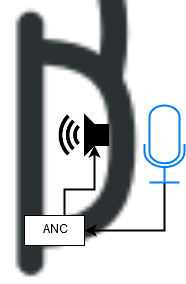
\includegraphics[scale=0.7]{../Assets/feedforward.png}
	\caption{Schemat układu aktywnego tłumienia typu feedforward.}
	\label{fig:feedforward}
\end{figure}

Zdecydowanie mocną stroną takiego rozwiązania jest fakt, iż mikrofon wyłapuje hałas wcześnie, co daje dostatecznie dużo czasu na wygenerowanie odpowiedzi. W~efekcie poprawia się nieco charakterystyka pracy układu w~zakresie wyższych częstotliwości.

Niestety, takie rozwiązanie jest praktycznie nie do przyjęcia -- układ nie ma możliwości sprawdzenia jakości odpowiedzi, zatem po jednorazowym nastrojeniu filtra przez konstruktora można doprowadzić do sytuacji, w~której niepoprawnie dopasowane słuchawki z~aktywnym tłumieniem hałasu mogą ten hałas wzmacniać, zamiast tłumić. Kolejną wadą jest również zewnętrzny montaż mikrofonu -- staje się bardziej wrażliwy na zakłócenia, takie jak wiatr, co mogło nie być wzięte pod uwagę w~laboratoryjnych warunkach konstrukcyjnych.
\subsection{Feedback}
\label{feedback}
\begin{figure}[h!]
	\centering
	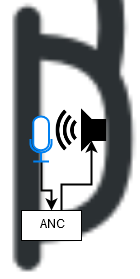
\includegraphics[scale=0.7]{../Assets/feedback.png}
	\caption{Schemat układu aktywnego tłumienia typu feedback.}
	\label{fig:feedback}
\end{figure}
To rozwiązanie jest dokładnie odwrotne niż poprzednie -- zamiast montować mikrofon na zewnątrz, montuje się go wewnątrz muszli (rys. \ref{fig:feedback}). Sprawia to, że mikrofon otrzymuje sygnał zbliżony do tego, który słyszy użytkownik. Otwiera to jednocześnie możliwość wprowadzenia systemu adaptacyjnego -- aby układ sam mógł dostrajać swoje parametry. Ta cecha oznacza równocześnie, że układ będzie znacznie mniej podatny na zakłócenia oraz niepoprawne założenie słuchawek.

Słabą stroną implementacji jest jednak fakt, że układ ma znacznie mniej czasu na przetworzenie sygnału i~wygenerowanie odpowiedzi, co sprawia, że zakres częstotliwości możliwych do wytłumienia zdecydowanie się obniża. W~skrajnym przypadku złego zaprojektowania układu, wadliwe ułożenie mikrofonu może spowodować destabilizujące sprzężenie zwrotne z~głośnikiem.
\subsection{Feedforward-Feedback -- układ hybrydowy}
\label{hybrid}
Aby zneutralizować wady wyżej wymienionych implementacji i~połączyć ich zalety, stosuje się ich połączenie hybrydowe -- układ feedforward-feedback (rys. \ref{fig:feedforward_feedback}). Mikrofon zewnętrzny generuje sygnał odpowiadający hałasowi z~otoczenia, co umożliwia tłumienie wyższych zakresów częstotliwości, zaś mikrofon wewnętrzny otwiera dla układu możliwość odsłuchu wygenerowanej odpowiedzi -- w~efekcie dając szansę na dostrojenie się do występujących warunków. 
\begin{figure}[h!]
	\centering
	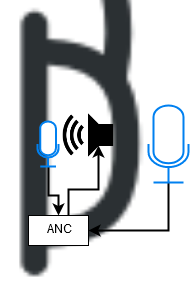
\includegraphics[scale=0.7]{../Assets/feedforward_feedback.png}
	\caption{Schemat układu aktywnego tłumienia typu feedforward-feedback.}
	\label{fig:feedforward_feedback}
\end{figure}

Wraz z~użyciem dwóch mikrofonów zwiększa się jednak znaczenie białego szumu w~elementach systemu. Aby zminimalizować to zjawisko, trzeba zastosować dobrej jakości komponenty, co szybko mnoży koszty takiego rozwiązania.
\subsection{Adaptacyjny algorytm filtracji}
\label{FIRLMS}
Warto postawić pytanie -- dlaczego dobrze jest zwiększyć cenę implementacji na rzecz otrzymania adaptacyjności systemu? Taka funkcjonalność pozwala na zwiększenie stabilności, trwałości oraz jakości systemu poprzez autokorektę parametrów zaimplementowanego filtra. Pozwala ona również na ustawiczne kompensowanie efektów starzenia komponentów systemu i~dostosowywanie się do zmiennych warunków zewnętrznych i~wewnętrznych. W~typowej konfiguracji sygnał z~mikrofonu zewnętrznego jest przepuszczany przez filtr i~podawany na wewnętrzny głośnik. Sygnały z obu mikrofonów -- wewnętrznego i~zewnętrznego -- są wykorzystywane do ustawicznego, adaptacyjnego dostrajania współczynników filtra tak, by wyciszyć wnętrze muszli nausznika. 

Autor użył filtra typu FIR, czyli Finite Impulse Response, co w~polskim przekładzie oznacza filtr o~skończonej odpowiedzi impulsowej. Zastosowano filtr rzędu 50. Algorytmem optymalizującym współczynniki filtra jest LMS, czyli Least-Mean-Squares -- realizuje on metodę najszybszego spadku. Typowy układ wspomniany przez autora przedstawiony jest na rysunku \ref{fig:typical_fir_lms}.
\begin{figure}[h!]
	\centering
	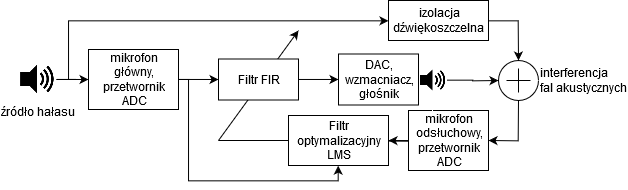
\includegraphics[width=\linewidth]{../Assets/typical_fir_lms.png}
	\caption{Typowy układ filtra adaptacyjnego do zastosowań tłumienia hałasu.}
	\label{fig:typical_fir_lms}
\end{figure}

Sygnał x'(n), który dochodzi do mikrofonu odsłuchowego, to ten sam hałas x(n), który słyszy mikrofon główny. Jest on jednak przekształcony przez środowisko, odległość oraz współczynnik pasywnego tłumienia materiałów użytych w~słuchawkach.

Sygnał wyjściowy, który generuje taki filtr, można obliczyć według następującego wzoru:\\
\begin{center} $ y(n) = \sum_{k=0}^{N-1} w_k(n)\cdot x(n-k) $ \end{center}
gdzie:\\
$y(n)$ -- sygnał wyjściowy w~\textit{n}-tej chwili czasu,\\
$N$ -- rząd filtra,\\
$w_k(n)$ -- wartość \textit{k}-tego współczynnika w~\textit{n}-tej chwili czasu,\\
$x(n-k)$ -- wartość sygnału wejściowego w~\textit{(n-k)}-tej chwili czasu.\\
Ponieważ filtr ma wiele~współczynników (jest rzędu wyższego niż pierwszy), to do obliczenia nowych wartości współczynników potrzebny jest gradient funkcji błędu średniokwadratowego. Zgodnie z~sugestią autora pozycji \cite{Chassaing}, można obliczyć estymatę nowego współczynnika używając gradientu funkcji $e^2(n)$ na podstawie niżej wspomnianego wzoru:\\
\begin{center} $ w_k(n+1) = w_k(n) + 2\cdot\beta\cdot e(n)\cdot x(n-k) \qquad k=0,1,\dots,N-1 $ \end{center}
gdzie:\\
$\beta$ -- współczynnik zbieżności filtra i~zarazem współczynnik jego dokładności,\\
$e(n)$ -- sygnał błędu (odsłuchowy).

Oczywiście zakres możliwości adaptacyjnych jest w~pewnym sensie uzależniony od platformy, na jakiej zrealizowany jest cały system -- co przedstawione będzie dokładniej w~następnym rozdziale.